% =============================================================================
% FILE NAME : 03_concept.tex
% DEPARTMENT: University of Tuebingen
% AUTOR     : Tom Schammo
% =============================================================================
% CONTENT   : Include for chapter "Concept"
% =============================================================================

The goal of this thesis is to implement keyword spotting on the UltraTrail architecture in Rust,
which relies on three components.
A microphone input, Mel Frequency Cepstral Coefficients (MFCC) \cite[Cha 2.5]{rust_pulp} to transform the audio to
a format that UltraTrail can work with and the UltraTrail drivers.
Figure~\ref{fig:pipeline} displays what the keyword-spotting process would look like.
First, there needs to be a sound source. Like a human speaking.
The microphone would pick that sound up, then after the MFCC features are extracted, they would serve
as an input for UltraTrail. UltraTrail would then determine if the audio picked up by the microphone
contains the desired keyword or not.

\begin{figure}[H]
    \centering
    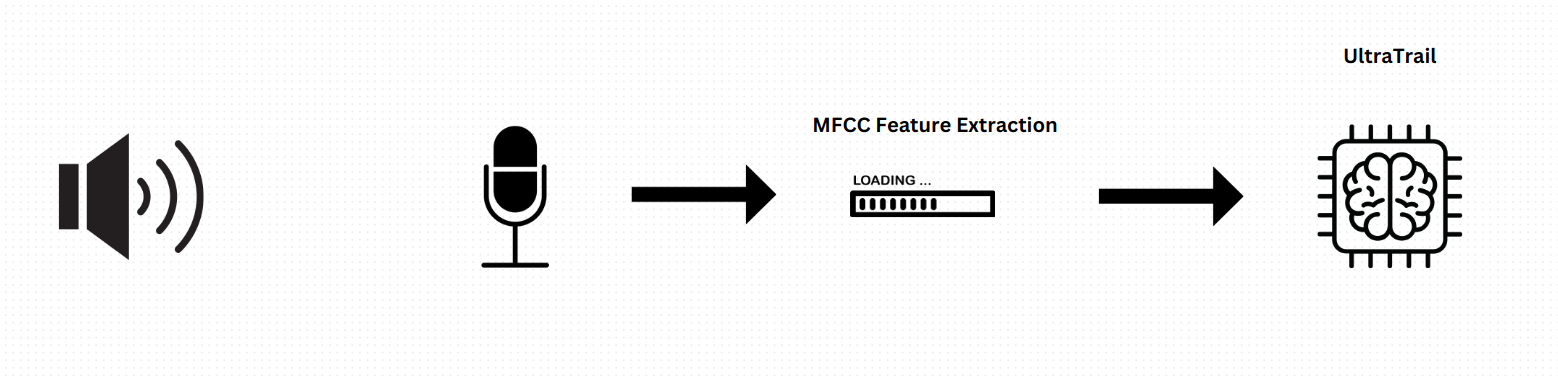
\includegraphics[width=0.9\textwidth]{figures/pipeline.png}
    \caption[Illustration of the keyword-spotting process]{Illustration of the keyword-spotting process}
    \label{fig:pipeline}
\end{figure}

One PDM and one $I^2S$ microphone have been selected, which exclusively use the $I^2S$ bus and were introduced
in chapter \ref{cha:fundamentals}.
To add support for the UltraTrail architecture and the microphones, the \lstinline{pulissimo_hal}
and \lstinline{pulissimo_pac} crates have to be expanded with drivers and example/test programs.
The PAC contains an SVD file that can be converted to Rust code to provide access to hardware registers
while the HAL crate provides the drivers and example programs for both UltraTrail and the microphones.
Drivers for $I^2S$ and PDM, as well as some example programs have already been implemented,
however neither have been tested nor run before.
Therefore, the implementations need to be tested and potentially modified.

\section{Experiments}

\subsection{Microphones}

To determine the functionality of the microphone, a sound that represents a perfect sine wave will be
played while the microphone is recording.
The output of the microphone should yield a perfect sine wave as well if it works as expected.\\
The data is analyzed using python scripts and plotted using pyplot\footnote{\url{https://matplotlib.org/stable/tutorials/introductory/pyplot.html}}.
A logic analyzer and oscilloscope are used as well to debug driver problems.

\subsection{UltraTrail}

The UltraTrail test makes sure that configuration changes have the desired effect (bits are correctly set in the correct registers),
and the AI accelerator is tested using a predefined set of input data.
After the input data is loaded correctly, the accelerator is started and will trigger a hardware-peripheral event when it is done.
After that, the results are compared with the desired results, which finally determines the functionality of the drivers.
